% Options for packages loaded elsewhere
\PassOptionsToPackage{unicode}{hyperref}
\PassOptionsToPackage{hyphens}{url}
\PassOptionsToPackage{dvipsnames,svgnames,x11names}{xcolor}
%
\documentclass[
  letterpaper,
  DIV=11,
  numbers=noendperiod]{scrartcl}

\usepackage{amsmath,amssymb}
\usepackage{iftex}
\ifPDFTeX
  \usepackage[T1]{fontenc}
  \usepackage[utf8]{inputenc}
  \usepackage{textcomp} % provide euro and other symbols
\else % if luatex or xetex
  \usepackage{unicode-math}
  \defaultfontfeatures{Scale=MatchLowercase}
  \defaultfontfeatures[\rmfamily]{Ligatures=TeX,Scale=1}
\fi
\usepackage{lmodern}
\ifPDFTeX\else  
    % xetex/luatex font selection
\fi
% Use upquote if available, for straight quotes in verbatim environments
\IfFileExists{upquote.sty}{\usepackage{upquote}}{}
\IfFileExists{microtype.sty}{% use microtype if available
  \usepackage[]{microtype}
  \UseMicrotypeSet[protrusion]{basicmath} % disable protrusion for tt fonts
}{}
\makeatletter
\@ifundefined{KOMAClassName}{% if non-KOMA class
  \IfFileExists{parskip.sty}{%
    \usepackage{parskip}
  }{% else
    \setlength{\parindent}{0pt}
    \setlength{\parskip}{6pt plus 2pt minus 1pt}}
}{% if KOMA class
  \KOMAoptions{parskip=half}}
\makeatother
\usepackage{xcolor}
\setlength{\emergencystretch}{3em} % prevent overfull lines
\setcounter{secnumdepth}{5}
% Make \paragraph and \subparagraph free-standing
\ifx\paragraph\undefined\else
  \let\oldparagraph\paragraph
  \renewcommand{\paragraph}[1]{\oldparagraph{#1}\mbox{}}
\fi
\ifx\subparagraph\undefined\else
  \let\oldsubparagraph\subparagraph
  \renewcommand{\subparagraph}[1]{\oldsubparagraph{#1}\mbox{}}
\fi


\providecommand{\tightlist}{%
  \setlength{\itemsep}{0pt}\setlength{\parskip}{0pt}}\usepackage{longtable,booktabs,array}
\usepackage{calc} % for calculating minipage widths
% Correct order of tables after \paragraph or \subparagraph
\usepackage{etoolbox}
\makeatletter
\patchcmd\longtable{\par}{\if@noskipsec\mbox{}\fi\par}{}{}
\makeatother
% Allow footnotes in longtable head/foot
\IfFileExists{footnotehyper.sty}{\usepackage{footnotehyper}}{\usepackage{footnote}}
\makesavenoteenv{longtable}
\usepackage{graphicx}
\makeatletter
\def\maxwidth{\ifdim\Gin@nat@width>\linewidth\linewidth\else\Gin@nat@width\fi}
\def\maxheight{\ifdim\Gin@nat@height>\textheight\textheight\else\Gin@nat@height\fi}
\makeatother
% Scale images if necessary, so that they will not overflow the page
% margins by default, and it is still possible to overwrite the defaults
% using explicit options in \includegraphics[width, height, ...]{}
\setkeys{Gin}{width=\maxwidth,height=\maxheight,keepaspectratio}
% Set default figure placement to htbp
\makeatletter
\def\fps@figure{htbp}
\makeatother
% definitions for citeproc citations
\NewDocumentCommand\citeproctext{}{}
\NewDocumentCommand\citeproc{mm}{%
  \begingroup\def\citeproctext{#2}\cite{#1}\endgroup}
\makeatletter
 % allow citations to break across lines
 \let\@cite@ofmt\@firstofone
 % avoid brackets around text for \cite:
 \def\@biblabel#1{}
 \def\@cite#1#2{{#1\if@tempswa , #2\fi}}
\makeatother
\newlength{\cslhangindent}
\setlength{\cslhangindent}{1.5em}
\newlength{\csllabelwidth}
\setlength{\csllabelwidth}{3em}
\newenvironment{CSLReferences}[2] % #1 hanging-indent, #2 entry-spacing
 {\begin{list}{}{%
  \setlength{\itemindent}{0pt}
  \setlength{\leftmargin}{0pt}
  \setlength{\parsep}{0pt}
  % turn on hanging indent if param 1 is 1
  \ifodd #1
   \setlength{\leftmargin}{\cslhangindent}
   \setlength{\itemindent}{-1\cslhangindent}
  \fi
  % set entry spacing
  \setlength{\itemsep}{#2\baselineskip}}}
 {\end{list}}
\usepackage{calc}
\newcommand{\CSLBlock}[1]{\hfill\break\parbox[t]{\linewidth}{\strut\ignorespaces#1\strut}}
\newcommand{\CSLLeftMargin}[1]{\parbox[t]{\csllabelwidth}{\strut#1\strut}}
\newcommand{\CSLRightInline}[1]{\parbox[t]{\linewidth - \csllabelwidth}{\strut#1\strut}}
\newcommand{\CSLIndent}[1]{\hspace{\cslhangindent}#1}

\KOMAoption{captions}{tableheading}
\makeatletter
\@ifpackageloaded{caption}{}{\usepackage{caption}}
\AtBeginDocument{%
\ifdefined\contentsname
  \renewcommand*\contentsname{Table of contents}
\else
  \newcommand\contentsname{Table of contents}
\fi
\ifdefined\listfigurename
  \renewcommand*\listfigurename{List of Figures}
\else
  \newcommand\listfigurename{List of Figures}
\fi
\ifdefined\listtablename
  \renewcommand*\listtablename{List of Tables}
\else
  \newcommand\listtablename{List of Tables}
\fi
\ifdefined\figurename
  \renewcommand*\figurename{Figure}
\else
  \newcommand\figurename{Figure}
\fi
\ifdefined\tablename
  \renewcommand*\tablename{Table}
\else
  \newcommand\tablename{Table}
\fi
}
\@ifpackageloaded{float}{}{\usepackage{float}}
\floatstyle{ruled}
\@ifundefined{c@chapter}{\newfloat{codelisting}{h}{lop}}{\newfloat{codelisting}{h}{lop}[chapter]}
\floatname{codelisting}{Listing}
\newcommand*\listoflistings{\listof{codelisting}{List of Listings}}
\makeatother
\makeatletter
\makeatother
\makeatletter
\@ifpackageloaded{caption}{}{\usepackage{caption}}
\@ifpackageloaded{subcaption}{}{\usepackage{subcaption}}
\makeatother
\ifLuaTeX
  \usepackage{selnolig}  % disable illegal ligatures
\fi
\usepackage{bookmark}

\IfFileExists{xurl.sty}{\usepackage{xurl}}{} % add URL line breaks if available
\urlstyle{same} % disable monospaced font for URLs
\hypersetup{
  pdftitle={Extraocular Motor Control (CNIII, IV, VI)},
  pdfauthor={Nathaniel Giovanni Yomogida, SPT; Chloë Anne Kerstein, SPT},
  colorlinks=true,
  linkcolor={blue},
  filecolor={Maroon},
  citecolor={Blue},
  urlcolor={Blue},
  pdfcreator={LaTeX via pandoc}}

\title{Extraocular Motor Control (CNIII, IV, VI)}
\author{Nathaniel Yomogida, SPT \and Chloë Kerstein, SPT}
\date{}

\begin{document}
\maketitle

\renewcommand*\contentsname{Table of contents}
{
\hypersetup{linkcolor=}
\setcounter{tocdepth}{3}
\tableofcontents
}
\section{Resources}\label{resources}

\begin{itemize}
\tightlist
\item
  Blumenfield Ch12,
  Ch13\textsuperscript{\citeproc{ref-blumenfeldNeuroanatomyClinicalCases2022}{1}}
\end{itemize}

\section{Overview}\label{overview}

\href{../../../../../../Alchemy\%20Archive/Neuro/Neuroanatomy/Cranial\%20Nerves/CN3_Oculomotor.qmd}{CN
III Oculomotor nerve},
\href{../../../../../../Alchemy\%20Archive/Neuro/Neuroanatomy/Cranial\%20Nerves/CN4_Trochlear.qmd}{CN
IV Trochlear Nerve}, and
\href{../../../../../../Alchemy\%20Archive/Neuro/Neuroanatomy/Cranial\%20Nerves/CN6_Abducens.qmd}{CN
VI Abducens Nerve} are responsible for controlling the
\href{../../../../../../Alchemy\%20Archive/Anatomy/OIANs/Extraocular\%20muscles/extraocular_muscles.qmd}{extraocular
muscles}\textsuperscript{\citeproc{ref-blumenfeldNeuroanatomyClinicalCases2022}{1}}.

\begin{itemize}
\tightlist
\item
  \href{../../../../../../Alchemy\%20Archive/Neuro/Neuroanatomy/Cranial\%20Nerves/CN6_Abducens.qmd}{CN
  VI Abducens Nerve} innervates the Lateral Rectus Muscle, which
  functions to abduct the eye laterally in the horizontal
  direction\textsuperscript{\citeproc{ref-blumenfeldNeuroanatomyClinicalCases2022}{1}}.
\item
  \href{../../../../../../Alchemy\%20Archive/Neuro/Neuroanatomy/Cranial\%20Nerves/CN4_Trochlear.qmd}{CN
  IV Trochlear Nerve} innervates the Superior Oblique muscle, which acts
  through a trochlea (pulley-like structure) to rotate the top of the
  eye medially and
  downward\textsuperscript{\citeproc{ref-blumenfeldNeuroanatomyClinicalCases2022}{1}}.
\item
  \href{../../../../../../Alchemy\%20Archive/Neuro/Neuroanatomy/Cranial\%20Nerves/CN3_Oculomotor.qmd}{CN
  III Oculomotor nerve} innervates all the other extraocular muscles to
  perform the rest of the eye's movements.
\end{itemize}

\subsection{Cranial Nerve Nuclei}\label{cranial-nerve-nuclei}

\begin{itemize}
\tightlist
\item
  The
  \href{../../../../../../Alchemy\%20Archive/Neuro/Neuroanatomy/Cranial\%20Nerves/Cranial\%20Nerve\%20Nuclei/oculomotor_nucleus.qmd}{oculomotor
  nucleus} (CN III) and the
  \href{../../../../../../Alchemy\%20Archive/Neuro/Neuroanatomy/Cranial\%20Nerves/Cranial\%20Nerve\%20Nuclei/trochlear_nucleus.qmd}{Trochlear
  nucleus} (CN IV) are located in the midbrain
\item
  The
  \href{../../../../../../Alchemy\%20Archive/Neuro/Neuroanatomy/Cranial\%20Nerves/Cranial\%20Nerve\%20Nuclei/abducens_nucleus.qmd}{abducens
  nucleus} (CN VI) is found in the
  pons\textsuperscript{\citeproc{ref-blumenfeldNeuroanatomyClinicalCases2022}{1}}.
\end{itemize}

\subsection{Nerve Pathways}\label{nerve-pathways}

\begin{figure}[H]

{\centering 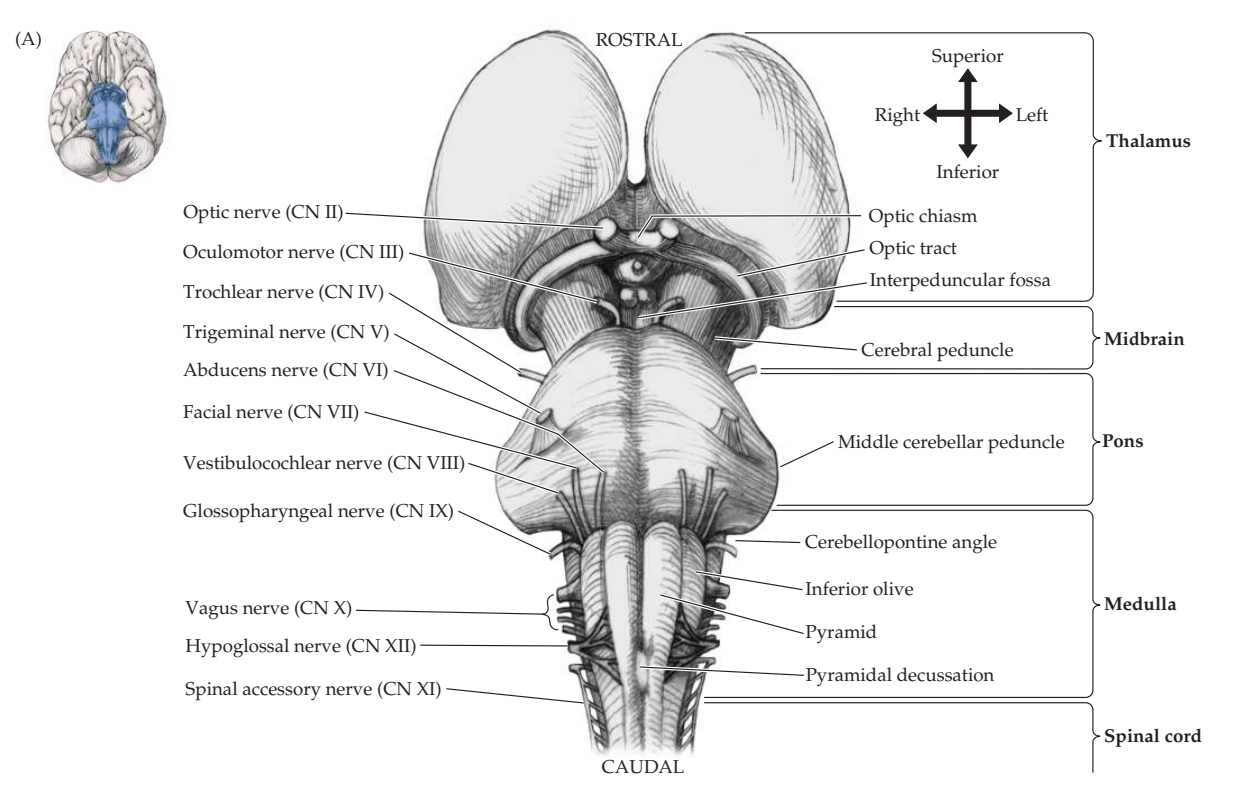
\includegraphics{../../../../../../Alchemy Archive/Neuro/Neuroanatomy/Cranial Nerves/images/fig12.2A Surface anatomy of the brainstem and cranial nerves blumenfield2022.png}

}

\caption{``Ventral view of Surface Anatomy of the brainstem and cranial
nerves (from fig12.2 of
Blumenfeld\textsuperscript{\citeproc{ref-blumenfeldNeuroanatomyClinicalCases2022}{1}})''}

\end{figure}%%
\begin{figure}[H]

{\centering 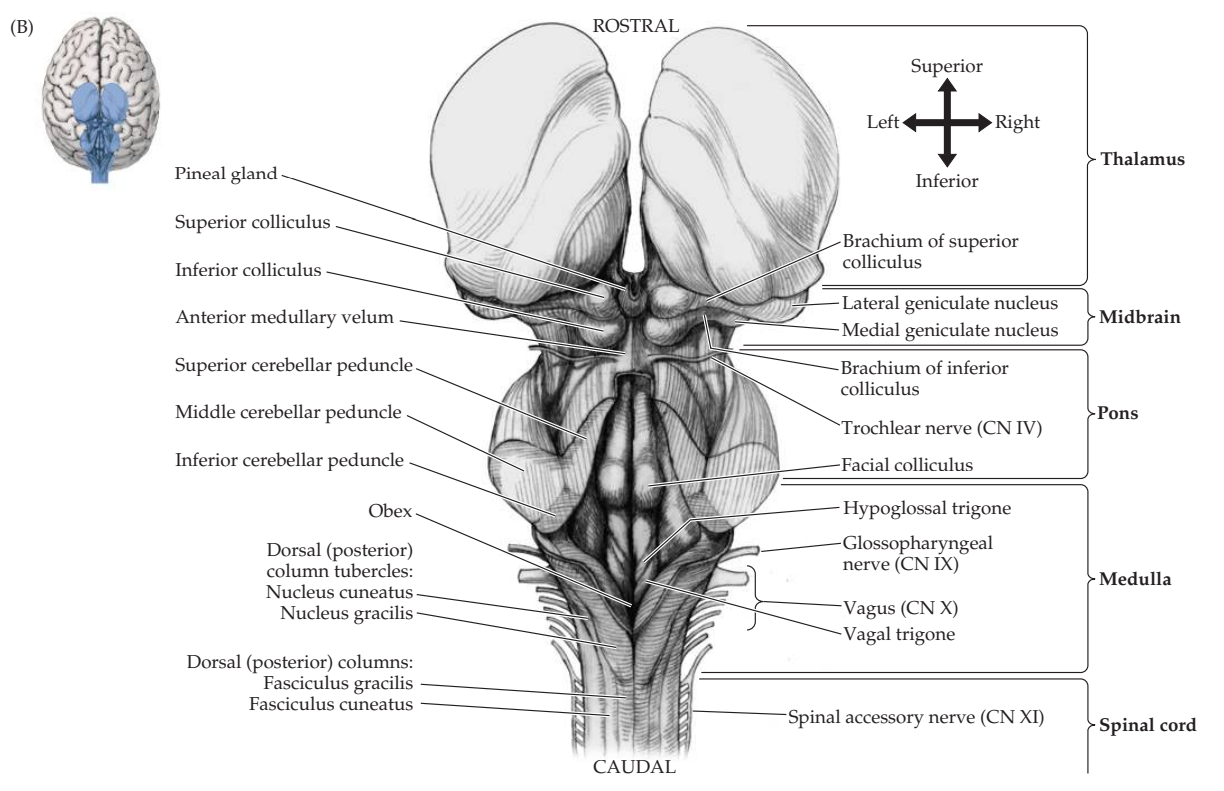
\includegraphics{../../../../../../Alchemy Archive/Neuro/Neuroanatomy/Cranial Nerves/images/fig12.2B Surface anatomy of the brainstem and cranial nerves blumenfield2022.png}

}

\caption{``Dorsal view of Surface Anatomy of the brainstem and cranial
nerves (from fig12.2 of
Blumenfeld\textsuperscript{\citeproc{ref-blumenfeldNeuroanatomyClinicalCases2022}{1}})''}

\end{figure}%%
\begin{figure}[H]

{\centering 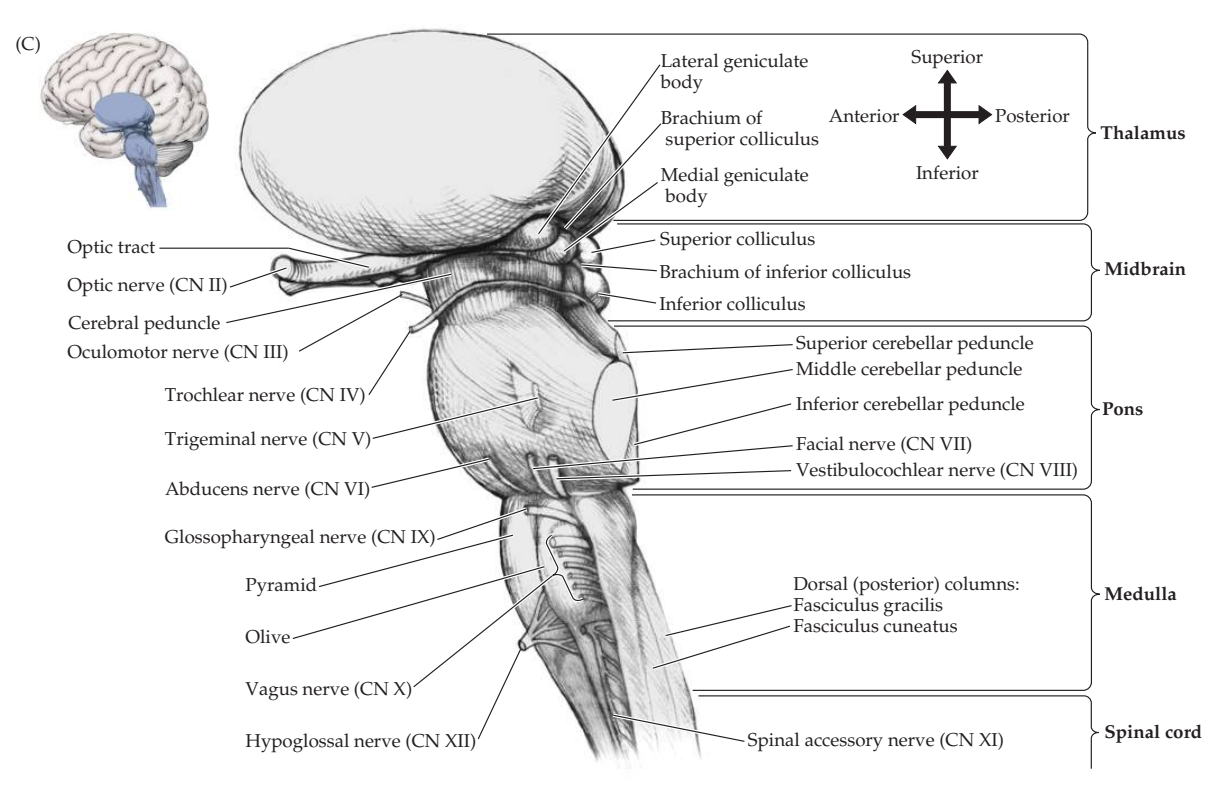
\includegraphics{../../../../../../Alchemy Archive/Neuro/Neuroanatomy/Cranial Nerves/images/fig12.2C Surface anatomy of the brainstem and cranial nerves blumenfield2022.png}

}

\caption{``Lateral view of the surface Anatomy of the brainstem and
cranial nerves (from fig12.2 of
Blumenfeld\textsuperscript{\citeproc{ref-blumenfeldNeuroanatomyClinicalCases2022}{1}})''}

\end{figure}%

\begin{itemize}
\tightlist
\item
  CN III exits the midbrain \textbf{ventrally} in the interpeduncular
  fossa\textsuperscript{\citeproc{ref-blumenfeldNeuroanatomyClinicalCases2022}{1}}.
\item
  CN IV exits the midbrain \textbf{dorsally} from the inferior
  tectum\textsuperscript{\citeproc{ref-blumenfeldNeuroanatomyClinicalCases2022}{1}}.
\item
  CN VI exits the pons ventrally at the pontomedullary
  junction\textsuperscript{\citeproc{ref-blumenfeldNeuroanatomyClinicalCases2022}{1}}.
  CN III, IV, and VI then traverse the cavernous sinus (see Figure
  13.11) and exit the skull via the superior orbital fissure (see Figure
  12.3A,C; Table 12.2) to reach the muscles of the orbit. CN III also
  carries parasympathetics to the pupillary constrictor and to the
  ciliary muscle of the lens. The preganglionic parasympathetic neurons
  are located in the EdingerWestphal nucleus in the midbrain (see Figure
  12.5). They synapse in the ciliary ganglion located in the orbit
  (Figure 12.6). Postganglionic parasympathetic fibers then continue to
  the pupillary constrictor and ciliary muscles. Other cranial nerve
  parasympathetics are also summarized in Figure 12.6.
\end{itemize}

\phantomsection\label{refs}
\begin{CSLReferences}{0}{1}
\bibitem[\citeproctext]{ref-blumenfeldNeuroanatomyClinicalCases2022}
\CSLLeftMargin{1. }%
\CSLRightInline{Blumenfeld H. \emph{Neuroanatomy Through Clinical
Cases}. 3rd ed. {Oxford university press}; 2022.}

\end{CSLReferences}



\end{document}
